\documentclass{bioinfo}
\copyrightyear{2008}
\pubyear{2008}

%\newif\ifnonbi
%\nonbifalse
%\newif\ifbi
%\bitrue


\begin{document}
\firstpage{1}

\begin{application}

\title[Infernal 1.0]{Infernal 1.0: inference of RNA alignments}
\author[E. Nawrocki, D. Kolbe and S. Eddy]{Eric P. Nawrocki,\,$^1$ Diana L. Kolbe\,$^1$ and Sean R. Eddy\,$^1$\footnote{to whom correspondence should be addressed}}
\address{$^{1}$HHMI Janelia Farm Research Campus, Ashburn VA 20147, USA\\}

\history{Received on XXXXX; revised on XXXXX; accepted on XXXXX}

\editor{Associate Editor: XXXXXXX}

\maketitle

%%%%%%%%%%%%%%%%%%%%%%%%%%%%%%%%%%%%%%%%%%%%%%%%%%%%%%%%%%%%%%%%%%%%%%%%%%%%%%%%%%%%%

\begin{abstract}
\section{Summary:}
\textsc{infernal} builds consensus RNA secondary structure profiles
called covariance models (CMs), and uses them to search nucleic acid
sequence databases for homologous RNAs, or to create new sequence- and
structure-based multiple sequence alignments.
\section{Availability:}
Source code, documentation, and benchmark downloadable from
http://infernal.janelia.org. \textsc{infernal} is freely
licensed under the GNU GPLv3 and should be portable to any
POSIX-compliant operating system, including Linux and Mac OS/X.
\section{Contact:} \{nawrockie,kolbed,eddys\}@janelia.hhmi.org
\end{abstract}

%%%%%%%%%%%%%%%%%%%%%%%%%%%%%%%%%%%%%%%%%%%%%%%%%%%%%%%%%%%%%%%%%%%%%%%%%%%%%%%%%%%%%

\section{Introduction}

When searching for homologous structural RNAs in sequence databases,
it is desirable to score both primary sequence and secondary structure
conservation.  The most generally useful tools that integrate sequence
and structure take as input any RNA (or RNA multiple alignment), and
automatically construct an appropriate statistical scoring system that
allows quantitative ranking of putative homologs in a sequence
database \citep{Gautheret01,ZhangBafna05,Huang08}.  Stochastic
context-free grammars (SCFGs) provide a natural statistical framework
for combining sequence and (non-pseudoknotted) secondary structure
conservation information in a single consistent scoring system
\citep{Sakakibara94c,Eddy94,Brown00,Durbin98}.

Here, we announce the 1.0 release of \textsc{infernal}, an
implementation of a general SCFG-based approach for RNA database
searches and multiple alignment. \textsc{infernal} builds consensus
RNA profiles called \emph{covariance models} (CMs), a special case of
SCFGs designed for modeling RNA consensus sequence and structure. It
uses CMs to search nucleic acid sequence databases for homologous
RNAs, or to create new sequence- and structure-based multiple
sequence alignments. One use of \textsc{infernal} is to annotate RNAs
in genomes in conjunction with the \textsc{Rfam} database
\citep{Gardner09}, which contains hundreds of RNA families.
\textsc{Rfam} follows a seed profile strategy, in which a
well-annotated ``seed'' alignment of each family is curated, and a CM
built from that seed alignment is used to identify and align
additional members of the family.  \textsc{infernal} has been in use
since 2002, but 1.0 is the first version that we consider to be a
reasonably complete production tool. It now includes E-value estimates
for the statistical significance of database hits, and heuristic
acceleration algorithms for both database searches and multiple
alignment that allow \textsc{infernal} to be deployed in a variety of
real RNA analysis tasks with manageable (albeit high) computational
requirements.

%%%%%%%%%%%%%%%%%%%%%%%%%%%%%%%%%%%%%%%%%%%%%%%%%%%%%%%%%%%%%%%%%%%%%%%%%%%%%%%%%%%%%

\section{Usage} 

A CM is built from a Stockholm format multiple sequence alignment (or
single RNA sequence) with consensus secondary structure annotation
marking which positions of the alignment are single stranded and which
are base paired \citep{infguide03}. CMs assign position specific
scores for the four possible residues at single stranded positions,
the sixteen possible base pairs at paired positions, and for
insertions and deletions. These scores are log-odds scores derived
from the observed counts of residues, base pairs, insertions and
deletions in the input alignment, combined with prior information
derived from structural ribosomal RNA alignments.  CM parameterization
has been described in more detail elsewhere
\citep{Eddy94,Eddy02b,KleinEddy03,infguide03,NawrockiEddy07}.

\textsc{infernal} is composed of several programs that are used in
combination by following four basic steps: 

\begin{enumerate}
\item Build a CM from a structural alignment with \emph{cmbuild}.
\item Calibrate a CM for homology search with \emph{cmcalibrate}.
\item Search databases for putative homologs with \emph{cmsearch}.
\item Align putative homologs to a CM with \emph{cmalign}.
\end{enumerate}

The calibration step is optional and computationally expensive (4
hours on a 3.0 GHz Intel Xeon for a CM of a typical RNA family of
length 100 nt), but is required to obtain E-values that estimate
the statistical significance of hits in a database
search. \emph{cmcalibrate} will also determine appropriate HMM filter
thresholds for accelerating searches without an appreciable loss of
sensitivity. Each model only needs to be calibrated once.

%%%%%%%%%%%%%%%%%%%%%%%%%%%%%%%%%%%%%%%%%%%%%%%%%%%%%%%%%%%%%%%%%%%%%%%%%%%%%%%%%%%%%

\section{Performance}

A published benchmark (independent of our lab) \citep{Freyhult07} and
our own internal benchmark used during development
\citep{NawrockiEddy07} both find that \textsc{infernal} and other CM
based methods are the most sensitive and specific tools for structural
RNA homology search among those tested. Figure~1 shows updated results
of our internal benchmark comparing \textsc{infernal} 1.0 to the
previous version (0.72) that was benchmarked in \citet{Freyhult07},
and also to family-pairwise-search with BLASTN \citep{Altschul97,
Grundy98b}.  \textsc{infernal}'s sensitivity and specificity have
greatly improved, due mainly to three relevant improvements in the
implementation \citep{infguide03}: a biased composition correction to
the raw log-odds scores, the use of Inside log likelihood scores (the
summed score of all possible alignments of the target sequence) in
place of CYK scores (the single maximum likelihood alignment score),
and the introduction of approximate E-value estimates for the scores.

The benchmark dataset used in Figure~1 includes query alignments and
test sequences from 51 \textsc{Rfam} (release 7) families (details in
\citep{NawrockiEddy07}).  No query sequence is more than 60\% identical
to a test sequence.  The 450 total test sequences were embedded at
random positions in a 10 Mb ``pseudogenome''.  Previously we generated
the pseudogenome sequence from a uniform residue frequency
distribution \citep{NawrockiEddy07}.  Because base composition biases
in the target sequence database cause the most serious problems in
separating significant CM hits from noise, we improved the realism of
the benchmark by generating the pseudogenome sequence from a 15-state
fully connected hidden Markov model (HMM) trained by
Baum-Welch expectation maximization \citep{Durbin98} on genome
sequence data from a wide variety of species.  Each of the 51 query
alignments was used to build a CM and search the pseudogenome, a
single list of all hits for all families were collected and ranked,
and true and false hits were defined (as described in
\citet{NawrockiEddy07}), producing the ROC curves in Figure~1.

\textsc{infernal} searches require a large amount of compute time (our
10 Mb benchmark search takes about 30 hours per model on average
(Figure~1)). To alleviate this, \textsc{infernal} 1.0 implements two
rounds of filtering.  When appropriate, the HMM filtering technique
described by \citet{WeinbergRuzzo06} is applied first with filter
thresholds configured by \emph{cmcalibrate} (occasionally a model with
little primary sequence conservation cannot be usefully accelerated by
a primary sequence-based filter as explained in \citep{infguide03}).  The
query-dependent banded (QDB) CYK maximum likelihood search algorithm
is used as a second filter with relatively tight bands ($\beta$=
$10^{-7}$, the $\beta$ parameter is the subtree length probability
mass excluded by imposing the bands as explained in
\citep{NawrockiEddy07}).  Any sequence fragments that survive the
filters are searched a final time with the Inside algorithm (again
using QDB, but with looser bands ($\beta$= $10^{-15}$)).  In our
benchmark, the default filters accelerate similarity search by about
30-fold overall, while sacrificing a small amount of sensitivity
(Figure~1). This makes version 1.0 substantially faster than
0.72. \textsc{BLAST} is still orders of magnitude faster, but
significantly less sensitive than \textsc{infernal}. Further
acceleration remains a major goal of \textsc{infernal} development.

The computational cost of CM alignment with \emph{cmalign} has been a
limitation of previous versions of \textsc{infernal}. Version 1.0 now
uses a constrained dynamic programming approach first developed by
\citet{Brown00} that uses sequence-specific bands derived from a
first-pass HMM alignment. This technique offers a dramatic speedup
relative to unconstrained alignment, especially for large RNAs such as
small and large subunit (SSU and LSU) ribosomal RNAs, which can now be
aligned in roughly 1 and 3 seconds per sequence, respectively, as
opposed to 12 minutes and 3 hours in previous versions.  This
acceleration has facilitated the adoption of \textsc{infernal} by RDP,
one of the main ribosomal RNA databases \citep{Cole09}.

\textsc{infernal} is now a faster and more sensitive tool for RNA
sequence analysis.  Version 1.0's heuristic acceleration techniques
make some important applications possible on a single desktop computer
in less than an hour, such as searching a prokaryotic genome for a
particular RNA family, or aligning a few thousand SSU rRNA sequences.
Nonetheless, \textsc{infernal} remains computationally expensive, and many
problems of interest require the use of a cluster.  The most expensive
programs (\emph{cmcalibrate}, \emph{cmsearch}, and \emph{cmalign}) are
implemented in coarse-grained parallel MPI versions which divide the
workload into independent units, each of which is run on a separate
processor. 

%%%%%%%%%%%%%%%%%%%%%%%%%%%%%%%%%%%%%%%%%%%%%%%%%%%%%%%%%%%%%%%%%%%%%%%%%%%%%%%%%%%%%

\section*{Acknowledgement}

We thank Goran Ceric for his peerless skill in managing Janelia Farm's
high performance computing resources.

\paragraph*{Funding\textcolon} 
\textsc{Infernal} development is supported by the Howard Hughes
Medical Institute. It has been supported in the past by an NIH NHGRI
training grant (T32-HG000045) to EPN, an NSF Graduate Fellowship to
DLK, NIH R01-HG01363, and a generous endowment from Alvin Goldfarb.


\begin{figure}[h]
\centerline{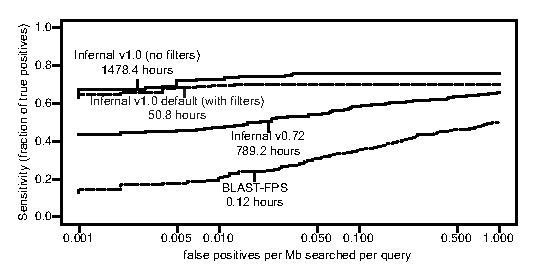
\includegraphics{roc-short}}
\caption{\textbf{ROC curves for the benchmark.}  Plots are shown for
the new \textsc{infernal} 1.0 with and without filters, for the old
\textsc{infernal} 0.72, and for family-pairwise-searches (FPS) with
\textsc{blastn}. CPU times are total times for all 51 family
searches measured for single execution threads on 3.0 GHz Intel Xeon
 processors. The \textsc{infernal} 1.0 times do not include time
 required for model calibration.}
\end{figure}


%%%%%%%%%%%%%%%%%%%%%%%%%%%%%%%%%%%%%%%%%%%%%%%%%%%%%%%%%%%%%%%%%%%%%%%%%%%%%%%%%%%%%
%
%     please remove the " % " symbol from \centerline{\includegraphics{fig01.eps}}
%     as it may ignore the figures.
%
%%%%%%%%%%%%%%%%%%%%%%%%%%%%%%%%%%%%%%%%%%%%%%%%%%%%%%%%%%%%%%%%%%%%%%%%%%%%%%%%%%%%%%

%\bibliographystyle{natbib}
%\bibliography{master,books,lab,new}

\begin{thebibliography}{}

\bibitem[Altschul {\em et~al.}(1997)Altschul, Madden, Schaffer, Zhang, Zhang,
  Miller, and Lipman]{Altschul97}
Altschul, S.~F., Madden, T.~L., Schaffer, A.~A., Zhang, J., Zhang, Z., Miller,
  W., and Lipman, D.~J. (1997).
\newblock Gapped {BLAST} and {PSI-BLAST}: A new generation of protein database
  search programs.
\newblock {\em Nucl. Acids Res.}, {\bf 25}, 3389--3402.

\bibitem[Brown(2000)Brown]{Brown00}
Brown, M.~P. (2000).
\newblock Small subunit ribosomal {RNA} modeling using stochastic context-free
  grammars.
\newblock {\em Proc. Int. Conf. Intell. Syst. Mol. Biol.}, {\bf 8}, 57--66.

\bibitem[Cole {\em et~al.}(2009)Cole, Wang, Cardenas, Fish, Chai, Farris,
  Kulam-Syed-Mohideen, McGarrell, Marsh, Garrity, and Tiedje]{Cole09}
Cole, J.~R., Wang, Q., Cardenas, E., Fish, J., Chai, B., Farris, R.~J.,
  Kulam-Syed-Mohideen, A.~S., McGarrell, D.~M., Marsh, T., Garrity, G.~M., and
  Tiedje, J.~M. (2009).
\newblock The {R}ibosomal {D}atabase {P}roject: Improved alignments and new
  tools for {rRNA} analysis.
\newblock in press.

\bibitem[Durbin {\em et~al.}(1998)Durbin, Eddy, Krogh, and Mitchison]{Durbin98}
Durbin, R., Eddy, S.~R., Krogh, A., and Mitchison, G.~J. (1998).
\newblock {\em Biological Sequence Analysis: Probabilistic Models of Proteins
  and Nucleic Acids\/}.
\newblock Cambridge University Press, Cambridge UK.

\bibitem[Eddy(2002)Eddy]{Eddy02b}
Eddy, S.~R. (2002).
\newblock A memory-efficient dynamic programming algorithm for optimal
  alignment of a sequence to an {RNA} secondary structure.
\newblock {\em BMC Bioinformatics\/}, {\bf 3}, 18.

\bibitem[Eddy(2003)Eddy]{infguide03}
Eddy, S.~R. (2003).
\newblock The {I}nfernal user's guide.
\newblock [http://infernal.janelia.org/].

\bibitem[Eddy and Durbin(1994)Eddy and Durbin]{Eddy94}
Eddy, S.~R. and Durbin, R. (1994).
\newblock {RNA} sequence analysis using covariance models.
\newblock {\em Nucl. Acids Res.}, {\bf 22}, 2079--2088.

\bibitem[Freyhult {\em et~al.}(2007)Freyhult, Bollback, and
  Gardner]{Freyhult07}
Freyhult, E.~K., Bollback, J.~P., and Gardner, P.~P. (2007).
\newblock Exploring genomic dark matter: A critical assessment of the
  performance of homology search methods on noncoding {RNA}.
\newblock {\em Genome Res.}, {\bf 17}, 117--125.

\bibitem[Gardner {\em et~al.}(2009)Gardner, Daub, Tate, Nawrocki, Kolbe,
  Lindgreen, Wilkinson, Finn, Griffiths-Jones, Eddy, and Bateman]{Gardner09}
Gardner, P.~P., Daub, J., Tate, J.~G., Nawrocki, E.~P., Kolbe, D.~L.,
  Lindgreen, S., Wilkinson, A.~C., Finn, R.~D., Griffiths-Jones, S., Eddy,
  S.~R., and Bateman, A. (2009).
\newblock Rfam: Updates to the {RNA} families database.
\newblock NAR, in press.

\bibitem[Gautheret and Lambert(2001)Gautheret and Lambert]{Gautheret01}
Gautheret, D. and Lambert, A. (2001).
\newblock Direct {RNA} motif definition and identification from multiple
  sequence alignments using secondary structure profiles.
\newblock {\em J. Mol. Biol.}, {\bf 313}, 1003--1011.

\bibitem[Grundy(1998)Grundy]{Grundy98b}
Grundy, W.~N. (1998).
\newblock Homology detection via family pairwise search.
\newblock {\em J. Comput. Biol.}, {\bf 5}, 479--491.

\bibitem[Huang {\em et~al.}(2008)Huang, Wu, Robertson, Feng, Malmberg, and
  Cai]{Huang08}
Huang, Z., Wu, Y., Robertson, J., Feng, L., Malmberg, R., and Cai, L. (2008).
\newblock Fast and accurate search for non-coding rna pseudoknot structures in
  genomes.
\newblock {\em Bioinformatics\/}, {\bf 24}, 2281--2287.

\bibitem[Klein and Eddy(2003)Klein and Eddy]{KleinEddy03}
Klein, R.~J. and Eddy, S.~R. (2003).
\newblock {RSEARCH:} finding homologs of single structured {RNA} sequences.
\newblock {\em BMC Bioinformatics\/}, {\bf 4}, 44.

\bibitem[Nawrocki and Eddy(2007)Nawrocki and Eddy]{NawrockiEddy07}
Nawrocki, E.~P. and Eddy, S.~R. (2007).
\newblock Query-dependent banding ({QDB}) for faster {RNA} similarity searches.
\newblock {\em PLoS Comput. Biol.}, {\bf 3}, e56.

\bibitem[Sakakibara {\em et~al.}(1994)Sakakibara, Brown, Hughey, Mian,
  Sj{\"{o}}lander, Underwood, and Haussler]{Sakakibara94c}
Sakakibara, Y., Brown, M., Hughey, R., Mian, I.~S., Sj{\"{o}}lander, K.,
  Underwood, R.~C., and Haussler, D. (1994).
\newblock Stochastic context-free grammars for {tRNA} modeling.
\newblock {\em Nucl. Acids Res.}, {\bf 22}, 5112--5120.

\bibitem[Weinberg and Ruzzo(2006)Weinberg and Ruzzo]{WeinbergRuzzo06}
Weinberg, Z. and Ruzzo, W.~L. (2006).
\newblock Sequence-based heuristics for faster annotation of non-coding {RNA}
  families.
\newblock {\em Bioinformatics\/}, {\bf 22}, 35--39.

\bibitem[Zhang {\em et~al.}(2005)Zhang, Haas, Eskin, and Bafna]{ZhangBafna05}
Zhang, S., Haas, B., Eskin, E., and Bafna, V. (2005).
\newblock Searching genomes for noncoding {RNA} using {FastR}.
\newblock {\em IEEE/ACM Trans. Comput. Biol. Bioinform.}, {\bf 2}, 366--379.

\end{thebibliography}

\end{application}

\end{document}
